\section{Desarrollo}

Cada método aproxima cada pixel de los $frames$ nuevos utilizando los pixeles de los $frames$ originales del video, y lo hace utilizando una función matemática. 
Por ejemplo, para generar el valor del pixel en la posición (i,j) de un nuevo $frame$, se utilizan los valores de los pixeles de los frames originales en la misma posicion (i,j). 

En el caso del método del vecino mas cercano hay solo dos valores posibles para un pixel. En los métodos lineal y cúbico ($splines$) se usan polinomios para hacer la aproximación.

\subsection{Método del vecino más cercano}
El algoritmo es bastante simple, cada $frame$ a agregar es la copia exacta del $frame$ original más cercano. Siendo $n$ la cantidad de $frames$ a agregar, cuando $n$ es par, se copia el frame $i$, $n/2$ veces y luego se copia el frame $i+1$ otras $n/2$. 

\begin{figure}[h!]
  \caption{Vecinos mas cercanos, agregando 2 frames}
  \centering
    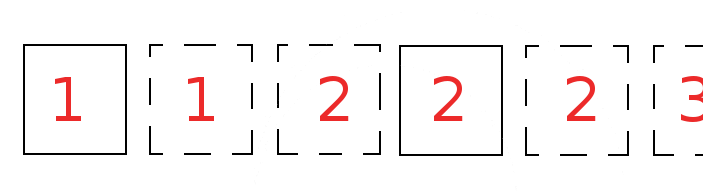
\includegraphics[width=0.5\textwidth]{imagenes/genCopypar.png}
\end{figure}

Cuando $n$ es impar, se copia el primer frame $n-1/2$ veces, y luego el resto de los frames se copia $n$ veces. Para el frame que está a igual distancia de los dos frames originales, utilizamos el frame posterior. No utilizamos ningún criterio en particular para esta decisión.

\begin{figure}[h!]
  \caption{Vecinos mas cercanos, agregando 3 frames}
  \centering
    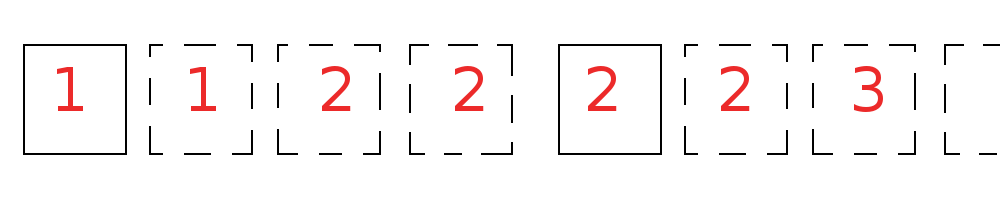
\includegraphics[width=0.5\textwidth]{imagenes/genCopyImpar.png}
\end{figure}

En las figuras anteriores, los cuadros con línea punteada son los frames interpolados, mientras que los frames con línea sin puntear son los frames originales.

\subsection{Método de interpolación lineal}
Se quiere aproximar con un polinomio de grado 1 (función lineal) los pixeles de los $frames$ que se agregan. Para estimar el valor del pixel $(i,j)$ en los nuevos frames, se utilizan los pixeles en la
misma posición $(i,j)$ de los $frames$ orginales anterior y posterior para construir el polinomio interpolador. \\

Si quisieramos agregar 2 frames nuevos, tomamos los valores del pixel en una posición determinada de los frames originales, que en el siguiente gráfico corresponde a los colores rojo y violeta, y a partir de ellos construimos una función lineal para averiguar los valores de los pixeles de los nuevos $frames$ (los de color azul y verde).


\begin{figure}[h!]
  \caption{Gráfico de los pixeles de los frames originales e interpolados}
  \centering
    
\includegraphics[width=0.5\textwidth]{imagenes/linealFrames.png}
\end{figure}

Con los valores de esas posiciones construimos una función lineal para determinar los valores intermedios que deberán tomar pixeles de los $frames$ interpolados.

\begin{figure}[h!]
  \caption{Funcion lineal de acuerdo a los valores entre dos pixeles}
  \centering
    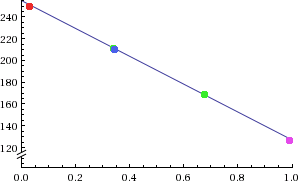
\includegraphics[width=0.5\textwidth]{imagenes/lineal2.png}
\end{figure}


El método equivale a encontrar los n-1 polinomios de primer grado $S_{j}$ que pasan por los puntos distintos $(x_{j},f(x_{j}))$ y $(x_{j+1},f(x_{j+1}))$ $\forall j \in (0,n-2)$.\\
En nuestro caso definimos los puntos $x_{0}, ... , x_{n-1}$ como el tiempo en que cada frame es reproducido. Por ejemplo, si tenemos un video a 24 fps, significa que en 1 segundo se muestran 24 frames. De este modo, sabemos que entre frame y frame hay una distancia temporal de 1/24 segundos. Estos son los valores que tomamos como los $x_{j}$ de nuestra función lineal. \\
Luego, ese intervalo se divide en intervalos equidistantes de acuerdo a la cantidad de frames que vayamos a agregar. Los valores $f(x_{j})$ equivalen al valor de un pixel del j-ésimo frame. 
%Es decir, se generan para cada pixel (i,j) de los n frames, n-1 polinomios.\\

%%%%%%%% imagen de toystory que explica lineal



\subsection{Interpolación cúbica o splines}
%SUPONEMOS QUE LA CANTIDAD DE FRAMES TOTALES (ORIGINALES) ES N+1, PARA QUE LOS ÍNDICES QUEDEN BONITOS.

Al igual que en el método de interpolación lineal, para las posiciones (i,j) de todos los frames del video, generamos los puntos intermedios a estos con splines, y asi generar las matrices de relleno posición a posición. Los $n+1$ puntos de interpolación $x_{0} .. x_{n}$ siguen representando el tiempo en el que cada frame es reproducido, dado por el framerate del video original.\\

Para construir los $n$ splines, se deben averiguar los valores de $4n$ constantes $a$, $b$, $c$ y $d$, correspondientes a los coeficientes de cada uno de los polinomios, con lo que se tiene bastante flexibilidad para asegurar que los splines construidos no solo son continuos y diferenciables en su intervalo, sino que tienen derivada segunda continua.\\
Primero recordaremos la definición de la interpolación cúbica por splines, para poder obtener propiedades a partir de ella: \\
Dada una función f: [a, b] y una sucesión de puntos $a= x_{0} < x_{1} < … < x_{n} = b$, una función interpolante cúbica S para f es una función que satisface las siguientes condiciones: \\

\begin{enumerate}
\item  S(x) es un polinomio de tercer grado, lo notamos como $S_{j}$ para el intervalo $[x_{j},x_{j+1}]$ $\forall j \in (0, n-1)$.
\item $S_{j}(x_{j})$ = $f(x_{j})$  y $S_{j}(x_{j+1})$ = $f(x_{j+1})$ $\forall j \int (0, n-1)$.
\item $S_{j+1}(x_{j+1})$ = $S_{j}(x_{j+1})$ $\forall j \in (0, n-2)$ (implicado por b)).
\item $S'_{j+1}(x_{j+1})$ = $S'_{j}(x_{j+1})$ $\forall j \in (0, n-2)$.
\item $S''_{j+1}(x_{j+1})$ = $S''_{j}(x_{j+1})$ $\forall j \in (0, n-2)$.
\item Alguna de las siguientes condiciones debe satisfacerse:
  \begin{enumerate}
  \item $S''(x_{0})$ = $S''(x_{n})$ = 0 (limite natural o libre).
  \item $S'(x_{0})$ = $f'(x_{0})$ y $S'(x_{n})$ = $f'(x_{n})$.
  \end{enumerate}
\end{enumerate}

En general la segunda condición del punto f) provee una aproximación más precisa porque incluye más información, sin embargo requeire los valores de la derivada de $f$ en los puntos de aproximación o una aproximación precisa de esos valores. Dado que no contamos con esta información, nos enfocamos en realizar un spline natural.\\


Construimos el spline aplicando las condiciones de la definición a los polinomios cúbicos\\ $S_{j}(x) = a_{j} + b_{j} (x - x_{j}) + c_{j} (x - x_{j})^{2} + d_{j} (x - x_{j})^{3}$ $\forall j \in (0, n-1)$.\\

Como $S_{j}$ = $a_{j}$ = $f(x_{j})$, la condición c) puede ser aplicada para obtener $ a_{j+1} = S_{j+1}(x_{j+1}) = S_{j}(x_{j+1}) = a_{j} + b_{j} (x_{j+1} - x_{j}) + c_{j} (x_{j+1} - x_{j})^{2} + d_{j} (x_{j+1} - x_{j})^{3}$ $\forall j \in (0, n-2)$.\\

Los términos $ x_{j+1} - x_{j} $ los renombraremos con la variable $h_{j}$ $\forall j \in (0, n-2)$ para mayor claridad. Si además llamamos $a_{n} = f(x_{n})$, entonces la ecuación

\begin{equation} \label{eq:ecuacion3.15}
a_{j+1} = a_{j} + b_{j} h_{j} + c_{j} h_{j}^{2} + d_{j} h_{j}^{3} 
\end{equation}

vale $\forall j \in (0, n-1)$. De manera similar, definiendo $b_{n} = S'(x_{n})$ se obtiene $S'_{j}(x) = b_{j} + 2c_{j} (x - x_{j}) + 3d_{j} (x - x_{j})^{2}$.
Si evaluamos en $x_{j}$ obtenemos  $S'_{j}(x_{j}) = b_{j}$, $\forall j \in (0, n-1)$. Si aplicamos la condición d) obtenemos

\begin{equation} \label{eq:ecuacion3.16}
b_{j+1} = b_{j} + 2c_{j} h_{j} + 3d_{j} h_{j}^{2}
\end{equation}

$\forall j \in (0, n-1)$. Otra relación entre los coeficientes de $S_{j}$ se obtiene definiendo $c_{n} = S''(x_{n})/2$ y luego aplicando la condición e). Tenemos que $\forall j \in (0, n-1)$ 

\begin{equation} \label{eq:ecuacion3.17}
c_{j+1} = c_{j} + 3d_{j} h_{j}.
\end{equation}

Despejando $d_{j}$ de la ecuación \ref{eq:ecuacion3.17} y reemplazando en las ecuaciones \ref{eq:ecuacion3.15} y \ref{eq:ecuacion3.16}, obtenemos que $\forall j \in (0, n-1)$ valen:\\

\begin{equation} \label{eq:ecuacion3.18}
a_{j+1} = a_{j} + b_{j} h_{j} + \frac{h_{j}^{2}}{3} (2c_{j} + c_{j+1})
\end{equation}
\begin{center} y \end{center}
\begin{equation} \label{eq:ecuacion3.19}
b_{j+1} = b_{j} + h_{j} (c_{j} + c_{j+1})
\end{equation}


Luego despejamos $b_{j}$ de la ecuación \ref{eq:ecuacion3.18} y reducimos el índice en uno, obteniendo 

\begin{equation} \label{eq:ecuacion3.20}
b_{j-1} = \frac{1}{h_{j-1}} (a_{j} - a_{j-1}) - \frac{h_{j-1}}{3} (2c_{j-1} + c_{j})                                
\end{equation}

Sustituimos $b_{j}$ y $b_{j-1}$ por sus valores correspondientes respecto a la ecuación \ref{eq:ecuacion3.19}. A continuación realizamos el despeje, para dar credibilidad a la cuestión:

$$b_{j} = b_{j-1} + h_{j-1} (c_{j-1} + c_{j})$$

$$\frac{1}{h_{j}} (a_{j+1} - a_{j}) - \frac{h_{j}}{3} (2c_{j} + c_{j+1}) = \frac{1}{h_{j-1}} (a_{j} - a_{j-1}) - \frac{h_{j-1}}{3} (2c_{j-1} + c_{j}) + h_{j-1} (c_{j-1} + c_{j})$$

$$ \frac{1}{h_{j}} (a_{j+1} - a_{j}) - \frac{1}{h_{j-1}} (a_{j} - a_{j-1}) = \frac{h_{j}}{3} (2c_{j} + c_{j+1}) - \frac{h_{j-1}}{3} (2c_{j-1} + c_{j}) + h_{j-1} (c_{j-1} + c_{j})$$

$$ \frac{3}{h_{j}} (a_{j+1} - a_{j}) - \frac{3}{h_{j-1}} (a_{j} - a_{j-1}) = h_{j} (2c_{j} + c_{j+1}) - h_{j-1} (2c_{j-1} + c_{j}) + 3h_{j-1} (c_{j-1} + c_{j}) $$

$$ \frac{3}{h_{j}} (a_{j+1} - a_{j}) - \frac{3}{h_{j-1}} (a_{j} - a_{j-1}) = 2h_{j}c_{j} + h_{j}c_{j+1} - 2h_{j-1}c_{j-1} - h_{j-1}c_{j} + 3h_{j-1}c_{j-1} + 3h_{j-1}c_{j} $$

$$ \frac{3}{h_{j}} (a_{j+1} - a_{j}) - \frac{3}{h_{j-1}} (a_{j} - a_{j-1}) = 2h_{j}c_{j} + h_{j}c_{j+1} + h_{j-1}c_{j-1} + 2h_{j-1}c_{j} $$

\begin{equation}\label{eq:ecuacion3.21}
 \frac{3}{h_{j}} (a_{j+1} - a_{j}) - \frac{3}{h_{j-1}} (a_{j} - a_{j-1}) = 2c_{j}(h_{j-1} + h_{j}) + h_{j-1}c_{j-1} + h_{j}c_{j+1} 
\end{equation}

$\forall j \in (1, n-1)$. \\

Las incógnitas de este sistema son los $\{c_{j}\}_{j=0}^{n}$. Los valores $\{ h_{j}\}_{j=0}^{n-1}$ y $\{ a_{j}\}_{j=0}^{n}$ están dados respectivamente por el espacio entre los puntos $\{x_{j}\}_{j=0}^{n}$ y los valores de f valuada en ellos. Una vez que los valores de $\{c_{j}\}_{j=0}^{n}$ son determinados, solo resta despejar $\{b_{j}\}_{j=0}^{n-1}$ de la ecuación \ref{eq:ecuacion3.20} y los $\{d_{j}\}_{j=0}^{n-1}$ de la ecuación \ref{eq:ecuacion3.17}. Con lo cual construimos los polinomios cúbicos $\{S_{j}(x)\}_{j=0}^{n-1}$. \\

El sistema planteado para buscar los valores $\{c_{j}\}_{j=0}^{n}$ los encuentra y además son únicos. La prueba de esto está formalizada en [BUR9].